\def\year{2019}\relax
%File: formatting-instruction.tex
\documentclass[letterpaper]{article} %DO NOT CHANGE THIS
\usepackage{aaai19}  %Required
\usepackage{times}  %Required
\usepackage{helvet}  %Required
\usepackage{courier}  %Required
\usepackage{url}  %Required
\usepackage{graphicx}  %Required
\usepackage{amssymb}
\usepackage{amsmath}
\usepackage[sort&compress,square,comma,authoryear]{natbib}

\usepackage{amsfonts}
\usepackage{amssymb}
\usepackage{amsthm}
\usepackage{bbm}
\usepackage{latexsym}
\usepackage{mathtools}
\usepackage{color}

\usepackage{algorithm}
\usepackage{algorithmic}


\frenchspacing  %Required
\setlength{\pdfpagewidth}{8.5in}  %Required
\setlength{\pdfpageheight}{11in}  %Required


%PDF Info Is Required:
  \pdfinfo{
/Title (2019 Formatting Instructions for Authors Using LaTeX)
/Author (AAAI Press Staff)}
\setcounter{secnumdepth}{0}  

\DeclareMathOperator*{\argmin}{argmin}
\DeclareMathOperator*{\argmax}{argmax}

\newcommand{\km}[1]{{\color{red} #1}} %red comments: Karsten
\newcommand{\wdb}[1]{{\color{blue} #1}} %blue comments: Walter

\begin{document}
% The file aaai.sty is the style file for AAAI Press 
% proceedings, working notes, and technical reports.
%
\title{Facility Location Utility for Uncovering Classifier Overconfidence}
\author{Karsten Maurer$^1$ \hspace{.2in} Walter Bennette$^2$\\
$^1$Miami University Department of Statistics - maurerkt@miamioh.edu\\ 
$^2$Air Force Research Lab Information Directorate - walter.bennette.1@us.af.mil \\
}

\maketitle
\begin{abstract}
AAAI creates proceedings, working notes, and technical reports directly from electronic source furnished by the authors. To ensure that all papers in the publication have a uniform appearance, authors must adhere to the following instructions. 
\end{abstract}

\section{Introduction}

Techniques such as active learning \citep{Settles2010} and domain adaptation \citep{Patel2014} can be used to create machine learning classifiers when large labeled datasets are not available for a specific task.  For example, the black box classifiers made available through many online services (Google Cloud, Amazon Web Services, etc) require no training data and can be thought of as a kind of domain adaptation.  However, with limited amounts of labeled data, users may not be able to properly evaluate a model, and are left hoping the model will be useful for their intended task.  In this paper we build upon previous work to develop an interactive method to help evaluate classifiers in the absence of labeled data.  Specifically, we develop an interactive method to uncover unknown unknowns \citep{Attenberg2015}: instances for which a classifier is confident in its prediction, but is wrong.  

Intuitive methods can be used to evaluate the performance of a model in the absence of labeled data.  For example, given a labeling budget one could sample instances following an experimental design, sample instances with the lowest classifier confidence, or sample instances identified as informative to the classifier through active learning strategies.  These methods could provide a sense of a model's performance but will potentially miss high confidence mistakes, referred to as \textit{unknown unknowns} (UUs).     

UUs can be thought of as blind spots to a classification model, and can be caused by dataset bias during training, domain shift during use, lack of model expressibility, and other causes of poor model fit.  From the viewpoint of a rational actor, UUs represent costly mistakes because minimal risk mitigation strategies will have been deployed for these high confidence predictions.  The discovery of UUs may allow new mitigation strategies to be formulated \citep{Nushi2016a}.  \wdb{Additionally, as enumerated in \citep{Bansal2018}, finding UUs is valuable to understand classifier limitations and prevent attacks (stole this hard)} \km{what do you mean by attacks?}

\citet{Attenberg2015} gamified the search for UUs and relied on human oracles to discover misclassified instances. A utility-based search algorithm for discovering UUs was then proposed by \citet{Lakkaraju2016} and expanded upon by \citet{Bansal2018}. In this paper, we propose a new utility function that shifts the emphasis from simply searching for UUs, to searching for UUs in areas of the model where errors occur more frequently than the model confidence would suggest, thus searching for classifier \textit{overconfidence}. 

\wdb{I enjoy a paragraph at the end that tells me what is coming in the rest of the paper. If we are short on space, or you disagree, that isn't necessary.} \km{Good idea, we should add this once we are certain what the rest of the paper contains}

\section{Previous Works}

\wdb{I think we need to introduce tau, and the fact that they are not necessarily using the classifier's own feature space}

\citet{Lakkaraju2016} define a utility model that counts the number of discovered UUs and searches for them with multi-armed bandits through a clustered feature space. \citet{Bansal2018} argued that this unit utility model motivates the discovery of very similar UUs. Instead, they propose an adaptive coverage-based utility model that attempts to encourage the discovery of high confidence UUs throughout a feature space. They then search for UUs via a greedy algorithm to maximize utility.

\begin{figure*}[h!]
  \centering
  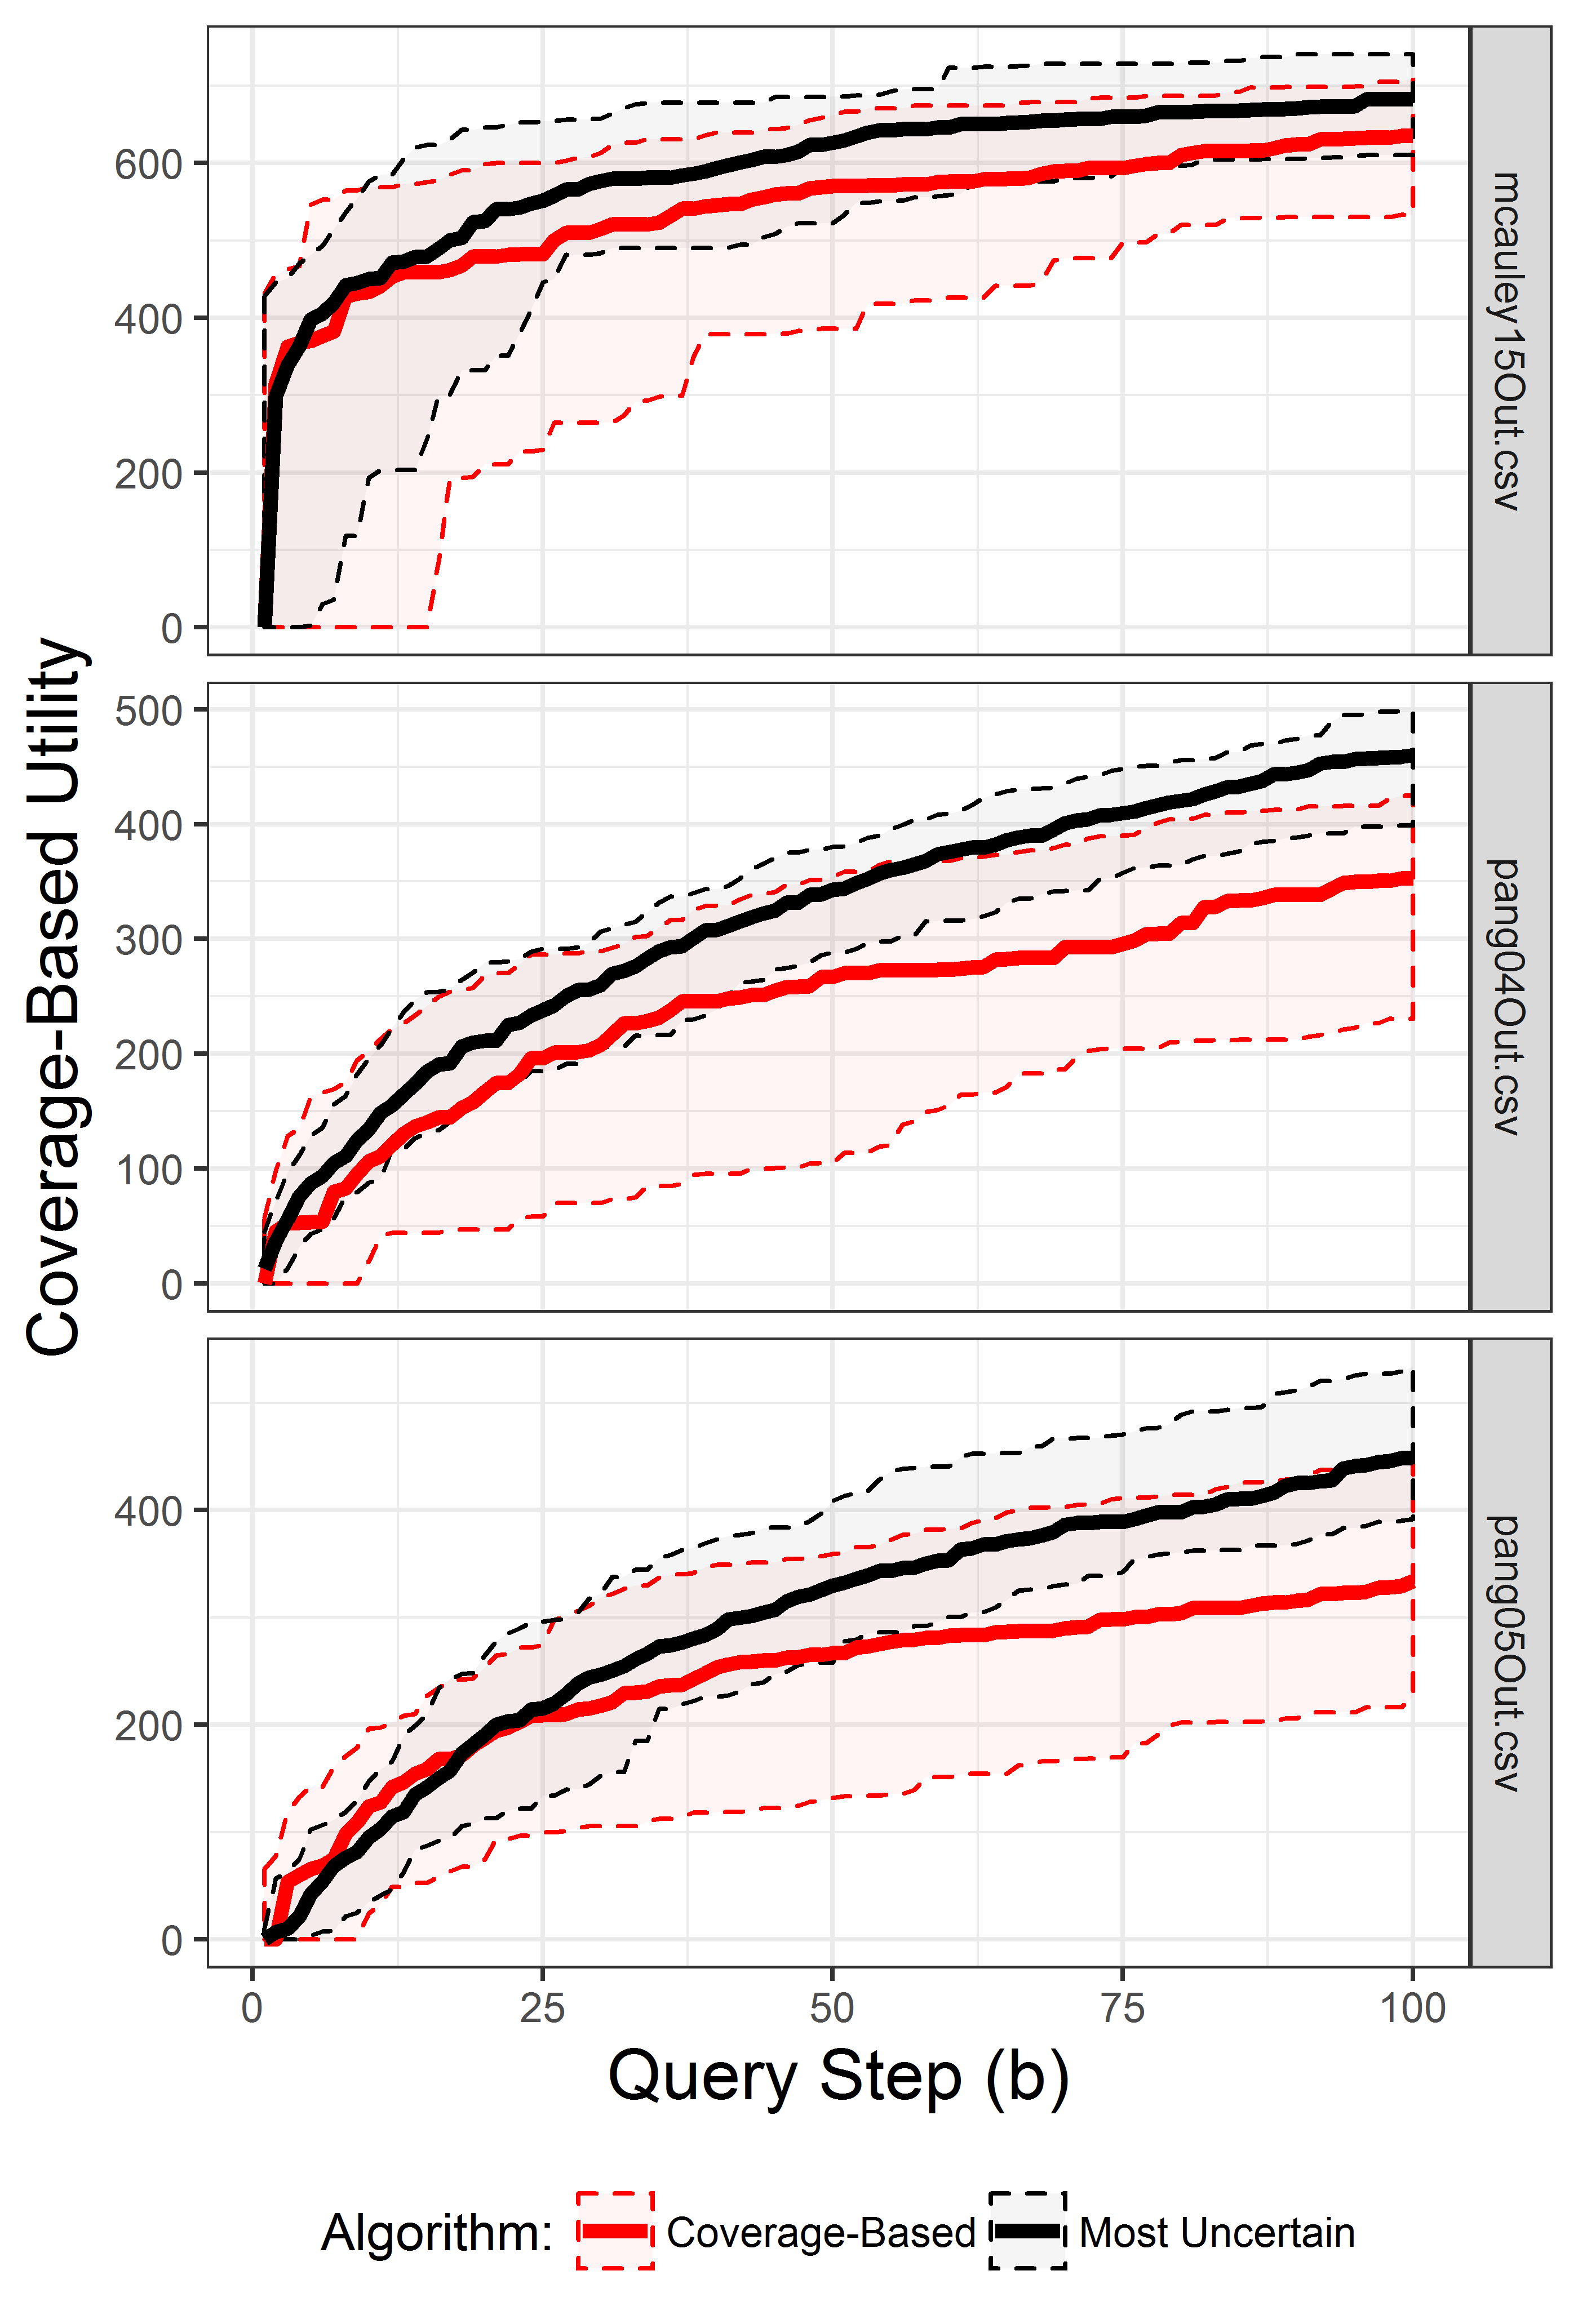
\includegraphics[width=\textwidth]{../experimentsAndPlots/CoverageVsMostUncertainPlaceholder.png}
  \caption{Empirical evidence that Coverage-Based Utility reward low confidence search.}
  \label{fig:coverutil}
\end{figure*}

\wdb{The utility model in \citet{Bansal2018} sums the prediction confidence of every test instance multiplied by a similarity measure to its closest discovered UU.}  It has the form: $$U(Q) = \sum_{x \in \mathbb{X}} c_x \cdot \max_{q \in S} \left\{sim\left(x,q \right) \right\}$$ where $\mathbb{X} \subset \mathbb{R}^p$ is the set of available $p$-dimensional unlabeled test instances, $Q \subset \mathbb{X}$ is the set of instances labeled by an oracle, $S = \left\{x|x \in Q, y_x \neq M(x)\right\}$ is the set of discovered UUs for some classifier $M(x):\mathbb{X} \rightarrow class$, $c_x$ is the classifier's confidence in its prediction of $x$, and $sim(x,q)$ is a distance based similarity metric. 

Given this utility model the search for UUs is performed by greedily selecting the instance $q'$ that maximizes the expected utility increase.  Meaning, $q'$ is selected to maximize, $$E\left[U_x\left(Q \cup q'\right)\right] = \hat{\phi}(x) \cdot c_x \cdot \max_{q \in S \cup q'} \left\{sim\left(x,q \right) \right\},$$ where $\hat{\phi}(x) = P\left(y_x \neq M(x) |Q \right)$ is a conditional probability that $x$ is misclassified given the query set.  As previously stated, this method is designed to incentivize a broader search for UUs and gives higher utility for finding misclassifications in higher confidence regions.  



Unfortunately, the method of \citet{Bansal2018} is consistently outperformed by sequentially querying instances for which the classifier is most uncertain. Query results were collected under the two search algorithms across 100 random samples of size n=1000 from each set of test data, with budget of B=100 quieries, because the greedy algorithms can unfold with high variability depending on the points gathered for testing. Figure~\ref{fig:coverutil} displays the Monte Carlo medians and 90\% confidence envelopes for the coverage-based utility for the four empirical data sets used in \citet{Bansal2018}. We see that the most-uncertain algorithm is typically given higher utility early in the algorithm than the results of the greedy-adaptive algorithm using the cluster-based probabilities to optimally select the next point.  We believe this exposes a flaw in the coverage-based utility model.  We see that the most-uncertain algorithm is typically given higher utility early in the algorithm than the results of the greedy-adaptive algorithm using the cluster-based probabilities to optimally select the next point. This reward strategy would help find high confidence UUs if instances with similar model prediction confidence scores were near each other in the feature space, but this does not seem to be the case.

\km{there is a lot of repetition here between then two blue paragraphs.}\wdb{Definitely a work in progress}

\wdb{Unfortunately, the coverage-based utility search of \citet{Bansal2018} consistently achieves lower utility than the simple strategy of sequentially querying instances for which the classifier is most uncertain.  This is shown in Figure~\ref{fig:coverutil} which displays Monte Carlo medians and 90\% confidence envelopes of the coverage-based utility for the four test datasets made available in \citet{Bansal2018}.  To account for the variability of the greedy search algorithms due to initial conditions, searches are performed following each strategy for 100 random samples of the test data of size n=1000, with a budget of B=100 queries.  We believe the superior performance of the most uncertain search exposes an issue in the coverage-based utility model.  

An issue with the coverage-based utility model is that it rewards the discovery of UUs near instances for which the classifier has high confidence, not the discovery of high confidence UUs themselves.  Therefore, the utility model may reward the discovery of low confidence mistakes more than the discovery of high confidence mistakes; the stated goal of the search. This is because there is no gaurantee that instances for which the classifier is similarly confident are confined to the same area of the feature space.  Meaning, it may be better to discover the easily found low confidence mistakes than the difficult to find high confidence mistakes. This is demonstrated by results shown in Figure~\ref{fig:coverutil}.  The most uncertain search (unsurprisingly) discovers more UUs than the coverage-based search, but if instances for which the classifier were similarly confident were confined to an area of the feature space, the additional discovery of UUs would not have lead to a drastic improvement of utility.

Given these apparent issues, we aim to construct a utility-based query algorithm that more appropriately rewards the identification of high confidence misclassifications, and helps to identify regions of classifier overconfidence.}



The coverage-based utility model attributes high utility for all high confidence points in the test set that are close to any discovered UU, thus attributing a utility to the uncertain status of non-queried points and even to points that have been confirmed by the oracle query to not be UU. Suppose that a single misclassified point exists in a region of high confident predictions, the utility would increase substantially for the surrounding points, despite not being UU. With these appearant issues, we aim to construct a utility-based query algorithm that more appropriately rewards the identification of high confidence misclassifications, and helps to identify regions of classifier overconfidence. 

\section{Methodology}

We propose an alternative utility model based roughly on facility location optimization methods  \km{(Farahani and Hekmatfar, 2009)}. In the facility location problem a utility can be constructed that uses a greedy algorithm to minimize the cost, or maximize the reward, of building a series of new facilities in a supply chain, while also minimizing distances between clients to the nearest facility  \km{(Guha and Khuller, 1999; Arya et al., 2004)}. In the UU query setting, we can draw an analog to the selection of a point to query to the establishment of a facility at that location in the feature space; evaluating the reward for selecting the point, and the distance it stands from the surrounding unobserved points. We propose a facility location utility function as: 

$$W(Q) = \sum_{x \in S} r \left(c_x\right) - \frac{1}{n} \sum_{x \in \mathbb{X}} \min_{q \in S}\left(d\left(x,q\right)\right)$$

where $r\left(c_x\right) = \log($1/$(1-c_x))$ is the reward function for finding an UU with confidence $c_{x}$, and $d(x,q)$ is the Euclidean distance between points $x$ and $q$. We use the greedy algorithm that at each iteration selects $q'$ with the maximum expected utility, as defined in Algorithm 1 below. 

%	FISTA with separation
\begin{algorithm}
	\caption{Greedy Facility Location Search}
	\label{alg:Greedy}
	\begin{algorithmic}
		\STATE {\bfseries Input:} Test set $\mathbb{X}$, prior $\hat{\phi}\left(x|Q=\emptyset\right)$, budget B
		\STATE $Q=\{\}$ \{inputs that have been queried\}
		\STATE $y_Q = \{\}$ \{oracle defined labels\}
		\STATE{\bfseries For: } $b = 1, 2, ..., B$ {\bfseries do:}

		\STATE $q' = \argmax_{q' \not\in Q} E \left[W\left(Q \cup q'\right) \right]$
		
		\STATE $y_{q'} = OracleQuery(q')$
		\STATE $Q \leftarrow Q \cup q'$
		\STATE $S \leftarrow \left\{x | x \in Q \space \text{ and } y_x \neq M(x) \right\}$
		\STATE $b \leftarrow b + 1$
			

		\STATE {\bfseries Return: $Q$ and $y_q$}
	\end{algorithmic}
\end{algorithm}

At each iterative step in Algorithm 1, we need to select the point that will maximize the expected gain in facility location utility, given probability estimates for point misclassification, such that  $\hat{\phi}(q' | Q) = \hat{P}(y_{q'} \ne M(q' ) |  Q )$. To find the expected gain in utility for each point, we evaluate the utility under the possibilities that the point is either misclassified or correctly classified. These possible utility outcomes are then averaged with weights equal to the estimated probability of each outcome. Thus the optimization step requires the solution of the following:

$$\underset{q' \notin Q}{argmax} E[W(Q \cup q')] = $$
\begin{equation*}
\small
\underset{q' \notin Q}{argmax} \left[\begin{split}
\hat{\phi}(q') \cdot \left[\sum_{x \in S \cup q'} r \left(c_x\right) - \frac{1}{n} \sum_{x \in \mathbb{X}} \min_{q \in S \cup q'}\left(d\left(x,q\right)\right) \right] + \\ 
(1-\hat{\phi}(q')) \cdot \left[\sum_{x \in S} r \left(c_x\right) - \frac{1}{n} \sum_{x \in \mathbb{X}} \min_{q \in S}\left(d\left(x,q\right)\right)\right]  
\end{split}\right]
\end{equation*}
\normalsize

Note that $\left[\sum_{x \in S} r \left(c_x\right) - \frac{1}{n} \sum_{x \in \mathbb{X}} \min_{q \in S}\left(d\left(x,q\right)\right)\right]$ is constant for all considered points, but cannot simply be removed from the argmax solution because it is multiplied by an estimated probability that is unique to each point. 

In addition to a change to the utility structure, we propose the use of model-based estimates for $\phi(x) = P\left(y_x \neq M(x) |Q \right)$. \citet{Bansal2018} use a multi-stage clustering procedure to create the estimates, $\hat{\phi}(x)$, that update after each new oracle query. The goal is to incorporate all new information into the evaluation the probabilistic structure in the optimization step of the greedy algorithm. This could alternatively be accomplished using model-based estimates, fit using the features and confidence scores of the query set to predict the chances of a misclassification. The posterior probabilty estimates that are common to most standard classification models provide a wide variety of options for creating the $\hat{\phi}(x)$ estimates. Without loss of generality, we demonstrate the use of logistic regression classifier probabilities, fitted such that:
$$\hat{\phi}(x) = logistic(c_x\hat{\beta}_0 + \sum_{j=1}^p x_j\hat{\beta}_j) = \frac{e^{c_x\hat{\beta}_0 + \sum_j x_j\hat{\beta}_j}}{1+e^{c_x\hat{\beta}_0 + \sum_j x_j\hat{\beta}_j}}$$
We select the logistic regression to demonstrate flexibility in estimating $\hat{\phi}(x)$ for several reasons: it is a generally familiar method, probabilities are the inherent model outputs, and it is computationally efficient to refit in the iterative query process. 

There are a few characteristics to note in the design of the facility locations utility model. First, the rewards are only accumulated by finding UUs in the query set, which avoids the issue of placing value on points in the test set for simply having high confidence points. Whereas having a small average minimum distance between all test points to the closest observed UU is also seen as valuable for encouraging strong coverage by the query set, especially early in the query sequence. 

The reward function is designed to impact the utility in a way that is consistent with a limiting factor being the budget for oracle queries. Viewed as a geometric distribution problem with a probability $\phi(x)$ of discovering a UU, we expect to need 1/$\phi(x)$ queried points like point $x$ before discovering the first UU \km{(Casella and Berger, 2002)}. For heuristic insight into the reward behavior construction, if we assume that   $\phi(x) ~= (1-c_x )$, then our reward is a log-scaled count of the number of randomly selected points we would expect to query in order to find the UUs in our query set. We use the log scaling to avoid over-incentivizing the search for incredibly rare UUs, as we know there is a limited budget for oracle queries. The optimization step will provide the highest expected rewards for selecting the most overconfident points relative to the updated probability estimates, that is to say when $(1-c_x )< \hat{\phi}(x)$. Note that unlike the UU definition, this construction does not depend on the arbitrary definition of a confidence threshold, $\tau$, beyond which we search for misclassifications. The reward component of the facility locations utility should encourage the query set to select any points where the model is most overconfident. We define \textit{overconfidence} as the difference between the confidence values given by the classifier and the actual rates of correct classification. 


\section{Experimental Evaluation}

We evaluate our facility location utility model by applying Algorithm 1 to four empirical data sets: pang04, pang05, mcauley15 and kaggle14. These sets originating from the \km{Pang and Lee (2004) movie review text classifier, Pang and Lee (2005) movie review text classifier, Mcauley et al. (2015) media review text classifier, and Kaggle (2014) “dogs-vs-cats” image classifier}, respectively. In each case we fit a classifier, $M(x)$, to a biased training set, then generate predicted classes and confidence values for all observations in the test set. Then singular value decomposition was used to reduce the dimensionality such that the test set, $\mathbb{X} \in \mathbb{R}^2$. The sets and classifiers were chosen to maintain consistency with the data used to evaluate methods in the previous works by Lakkaraju et al. (2017) and Bansal and Weld (2018). The pang04, pang05 and Mcauley15 sets come directly from the generously shared repository accompanying the work Bansal and Weld (2018). \km{The construction of the kaggle14 training set, test set and classifier....}

\begin{figure}[hbtp]
  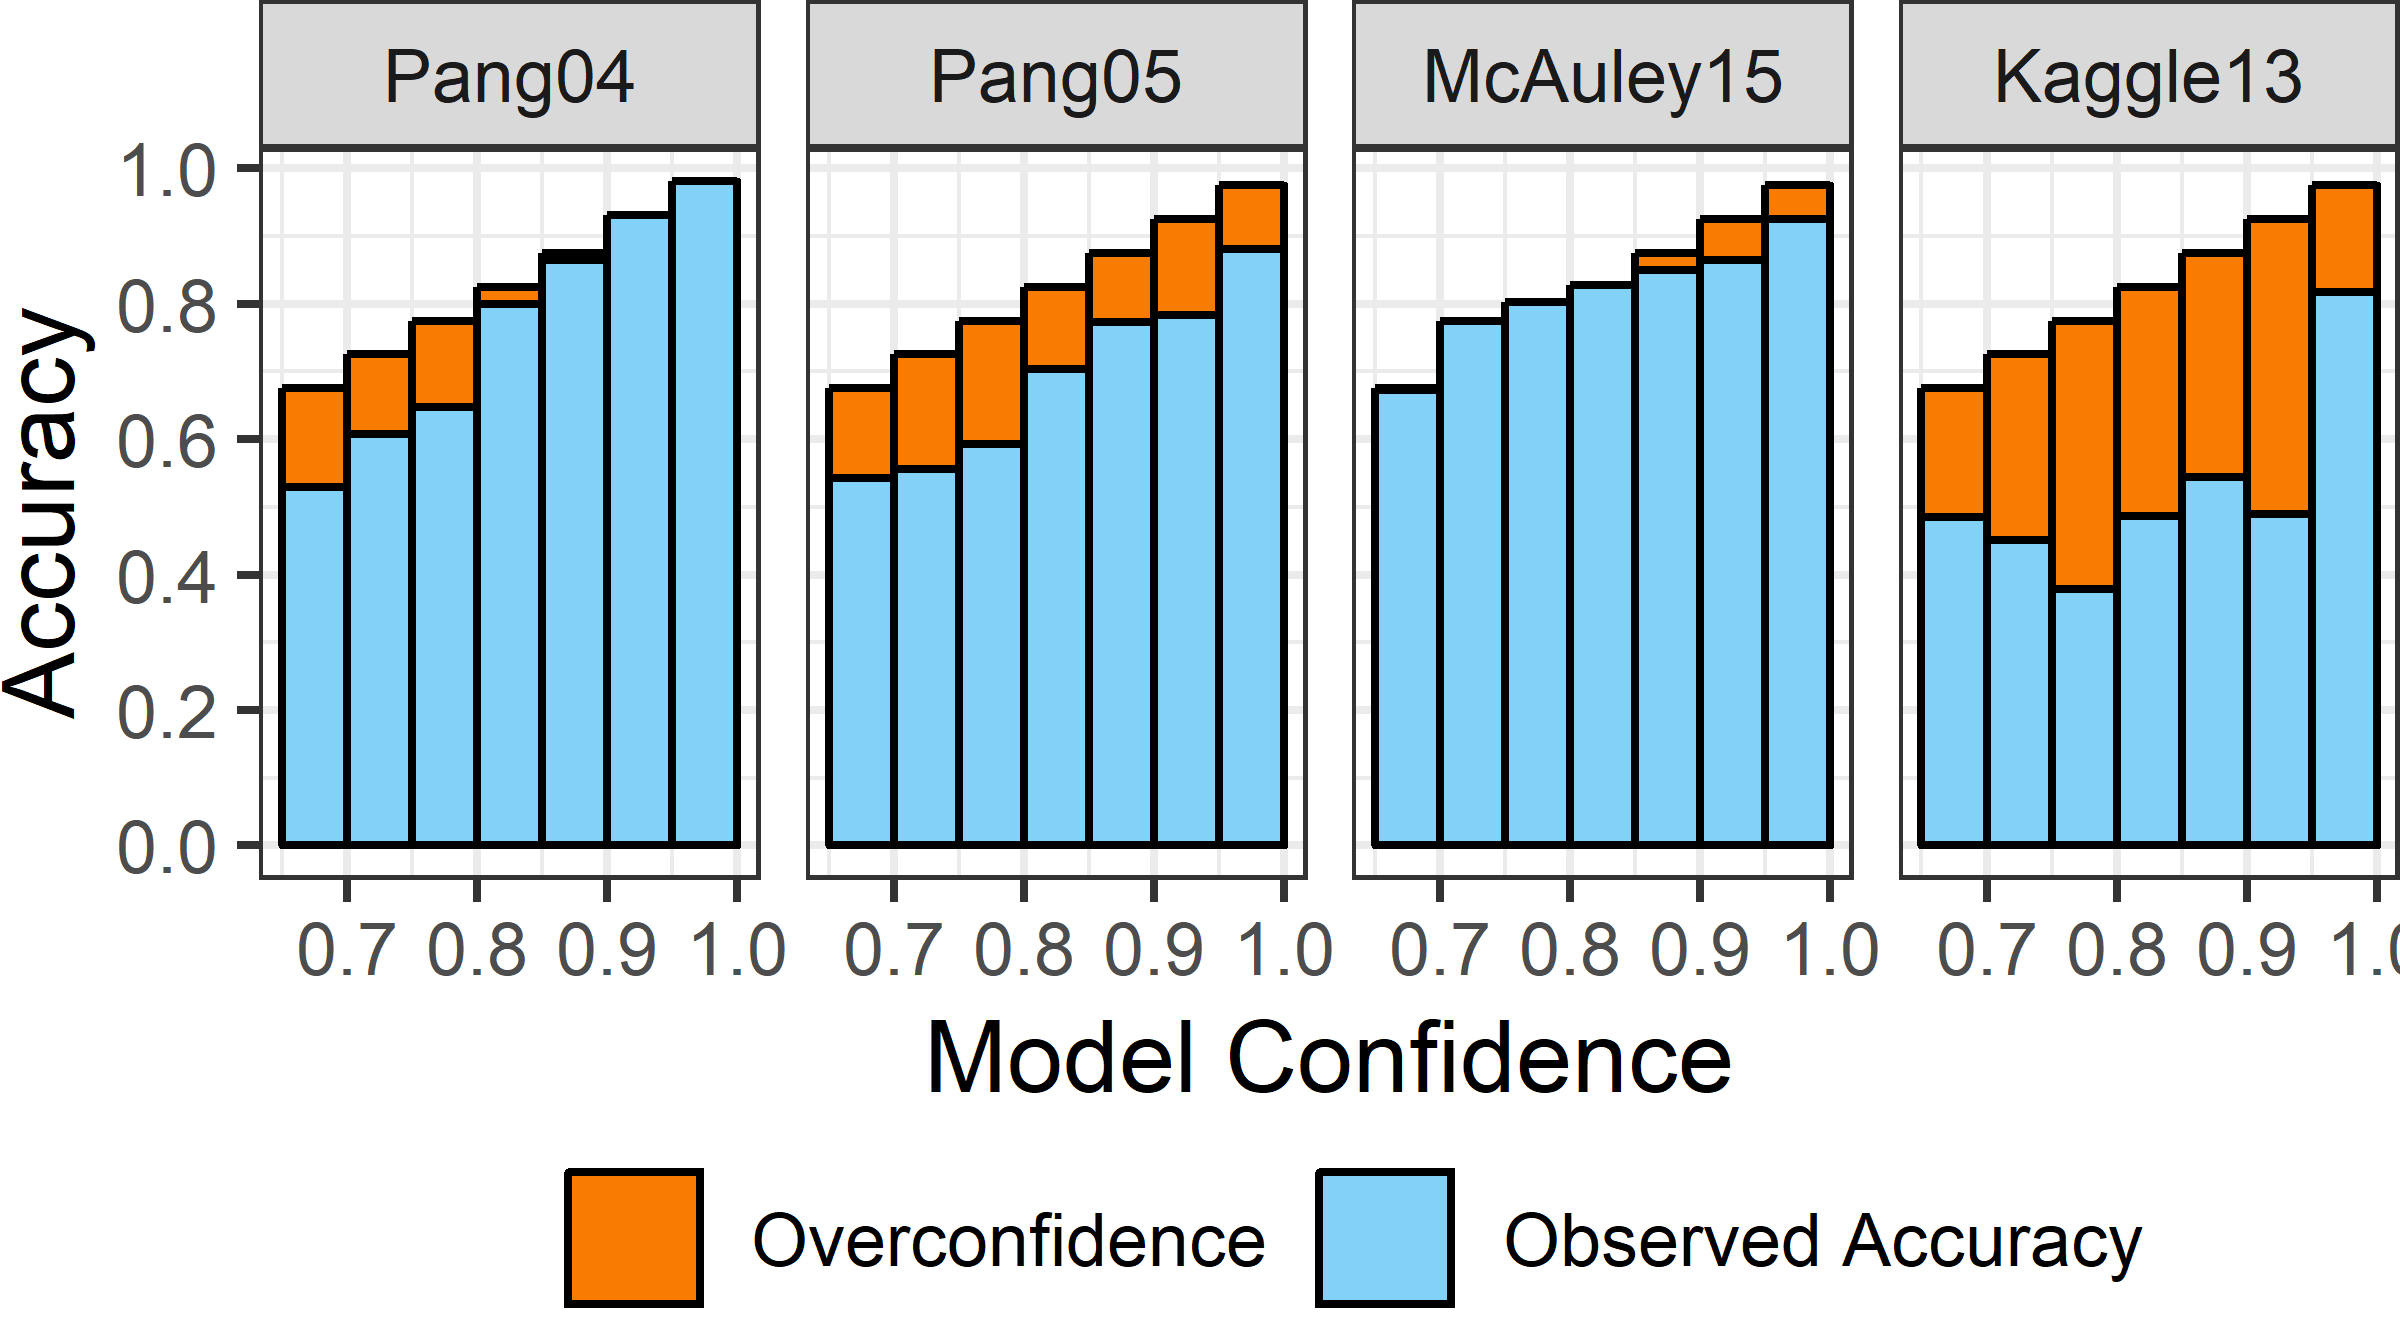
\includegraphics[width=.45\textwidth]{../experimentsAndPlots/overconfidence.png}
  \caption{Observed overconfidence of the model for experimental data sets.}
  \label{fig:overconf}
\end{figure}

Figure~\ref{fig:overconf} displays the overconfidence of the models using a cubic-splines fitted between the indicator of correct classification an the confidence value in each test dataset to obtain an empirical estimates of the true rates of correct classification. We see that the models from the Pang04 and Pang05 datasets are most overconfident for points with relatively low confidence values, thus we would expect the a simple sequential search of the most-uncertain points to provide high facility locations utility in these cases. Whereas the predictions for McCauley15 and Kaggle14 are most overconfident in the highest confidence range, thus the most-uncertain search should provide low facility locations utility in these cases. We see that these four data sets represent fairly different profiles of overconfidence, thus present good variety for evaluating characteristics of the facility locations utility model. 


To evaluate the queries generated by the facility locations utility model we collect query results from running Algorithm~\ref{alg:Greedy} on repeated random samples from the test sets, thus allowing Monte Carlo estimates for utility characteristics. The optimization step was completed using both the logistic regression and the cluster-based construction of the probability estimates, $\phi(x)$. Figure 2 displays the Monte Carlo medians and 90\% confidence envelopes for the utility gains, paired with a visualization of confidence ranges where the model most overestimates its accuracy. To allow meaningful comparison over different test sets, that performance is scaled relative to the tractable upper bound – obtained by running the greedy algorithm with an omniscient knowledge of test misclassification. 

\begin{figure*}[t]
 \centering
  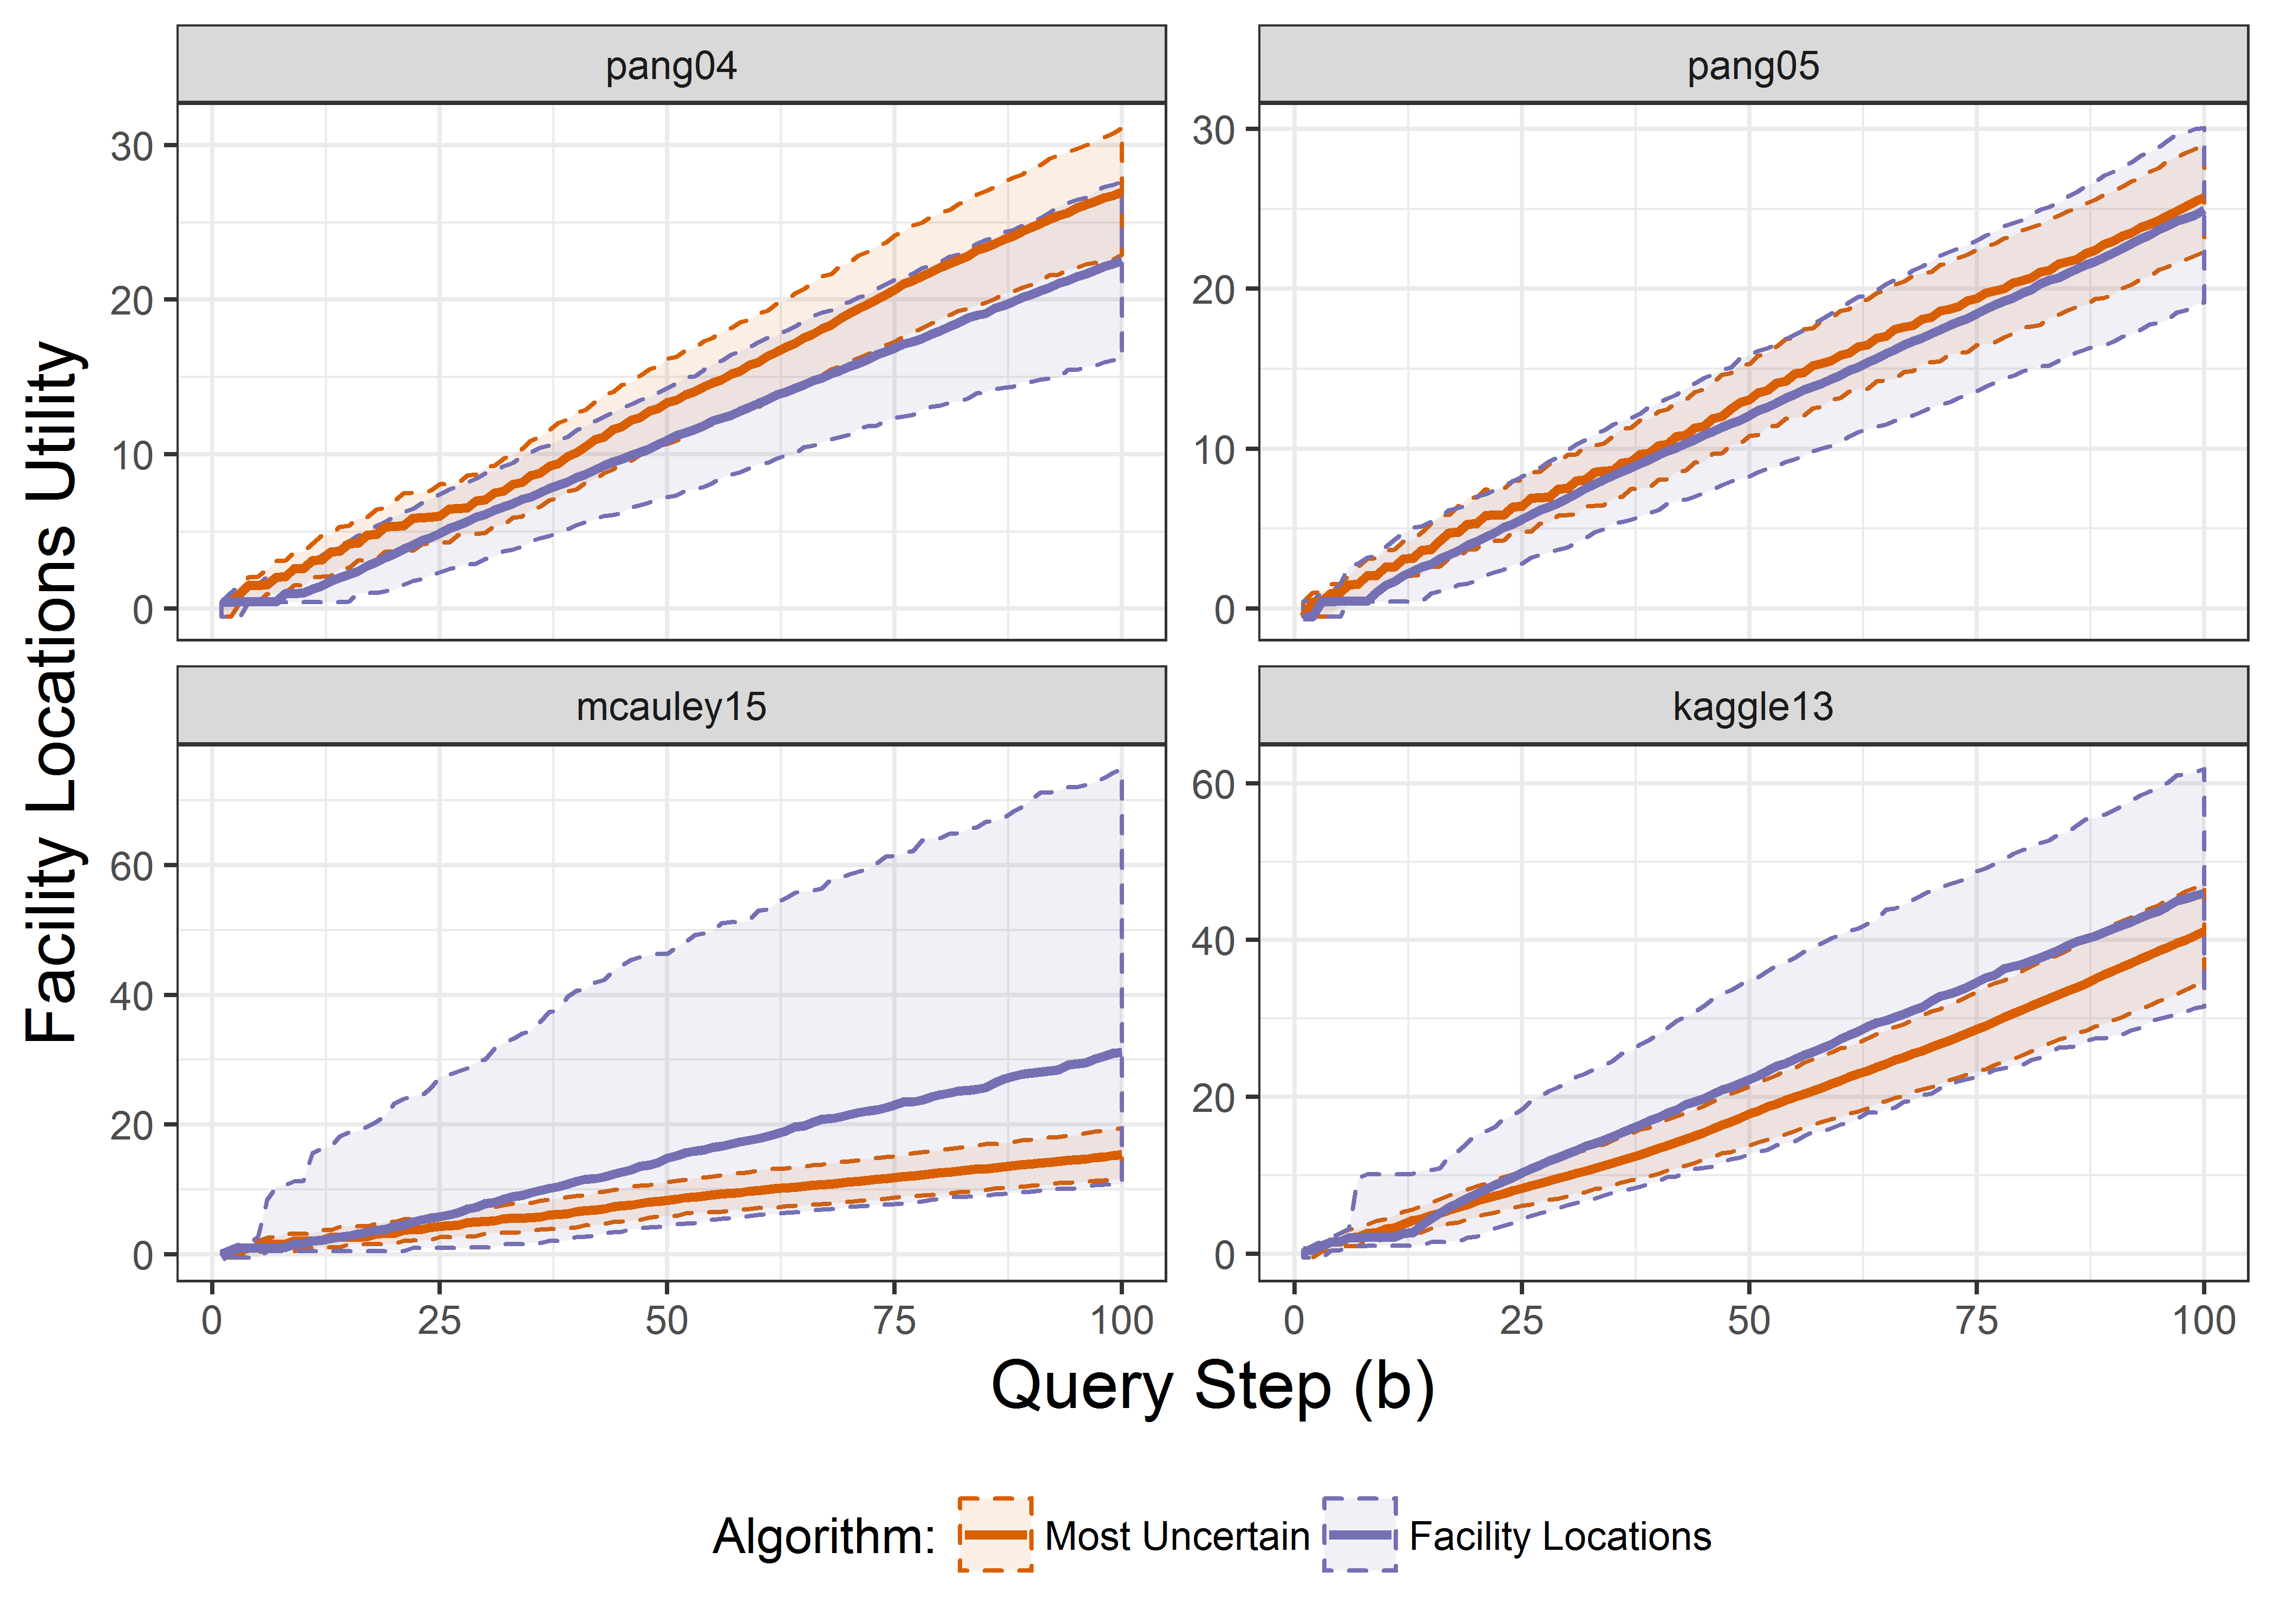
\includegraphics[width=\textwidth]{../experimentsAndPlots/flUtilPlaceholder.png}
  \caption{Faciltiy Locations Utility rewards finding overconfidence}
  \label{fig:flutil}
\end{figure*}

In Figure~\ref{fig:flutil}, we see that the most-uncertain selection method – that begins its search with points with confidence values just above $\tau$=.65 – provides the strongest utility for the pang04 case, as is desired, because these points are also shown to be most overconfident. The facility locations utility outcomes from using the logistic-based optimization were typically slightly lower. For the pang05 case where the overconfidence is skewed right but relatively ubiquitous, we again find very comparable utility between the logistic-based and the most-uncertain queries. For the mcauley15 where overconfidence is heavily skewed left, we now see inconsistent but strong facility location utility outcomes from the facility locations search, and consistently low utility outcomes from the most-uncertain queries. \km{In the last case of kaggle14 where the overconfidence is skewed left but relatively ubiquitous, the facility locations search provided less consistent, but typically stronger utility than most-uncertain searches}. 

We also look to compare the queries gathered by the coverage-based utility algorithm and facility locations utility algorithm. Given that both rely on greedy selection relative to their own utility function, it does not make sense to compare their selections on the utility values directly. Instead we compare the efficiency of the search for UUs, using a summary statistics that we call the \textit{standardized discovery ratio} (SDR). The SDR is an adaptation of the \textit{standardized mortality ratio} used in biostatistics to evaluate the mortality rate for a given sample of patients, which standardizing using their initial risk of death (\km{Bernard and Rosner, 1990; Taylor, 2013}). In our case we use an analog that evalues the misclassification rate, standardized by the initial model confidence. The SDR for a set of queried points is computed as
$$ ||S|| / \sum_{x=1}^B(1- c_x) $$
thus counting the number of discovered misclassifications, divided by the number of misclassifications expected given the confidence values of the points queried. The SDR can be interpreted as the number of time more misclassifications that were found than were expected based on model confidence, allowing for fair compare the efficiency of queries from any search method. \km{In Table~\ref{tab:sdr} we see... }

% latex table generated in R 3.4.1 by xtable 1.8-2 package
% Tue Aug 21 09:33:32 2018
\begin{table}[ht]
\centering
\begin{tabular}{llll}
  \hline
dataset & Most Uncertain & Coverage-Based & Facility Locations \\ 
  \hline
pang04 & 1.53 (1.33,1.71) & 1.47 (1.23,1.67) & 1.43 (1.14,1.69) \\ 
  pang05 & 1.41 (1.21,1.56) & 1.66 (1.35,2.06) & 1.54 (1.16,2.08) \\ 
  mcauley15 & 0.89 (0.71,1.08) & 1.09 (0.83,1.61) & 1.27 (0.76,8.08) \\ 
  kaggle14 & 2.55 (2,3.02) & 3.09 (2.33,4.26) & 3.58 (2.52,4.99) \\ 
   \hline
\end{tabular}
  \caption{Standardized Discovery Ratio.}
  \label{tab:sdr}
\end{table}


\begin{figure}[hbtp]
  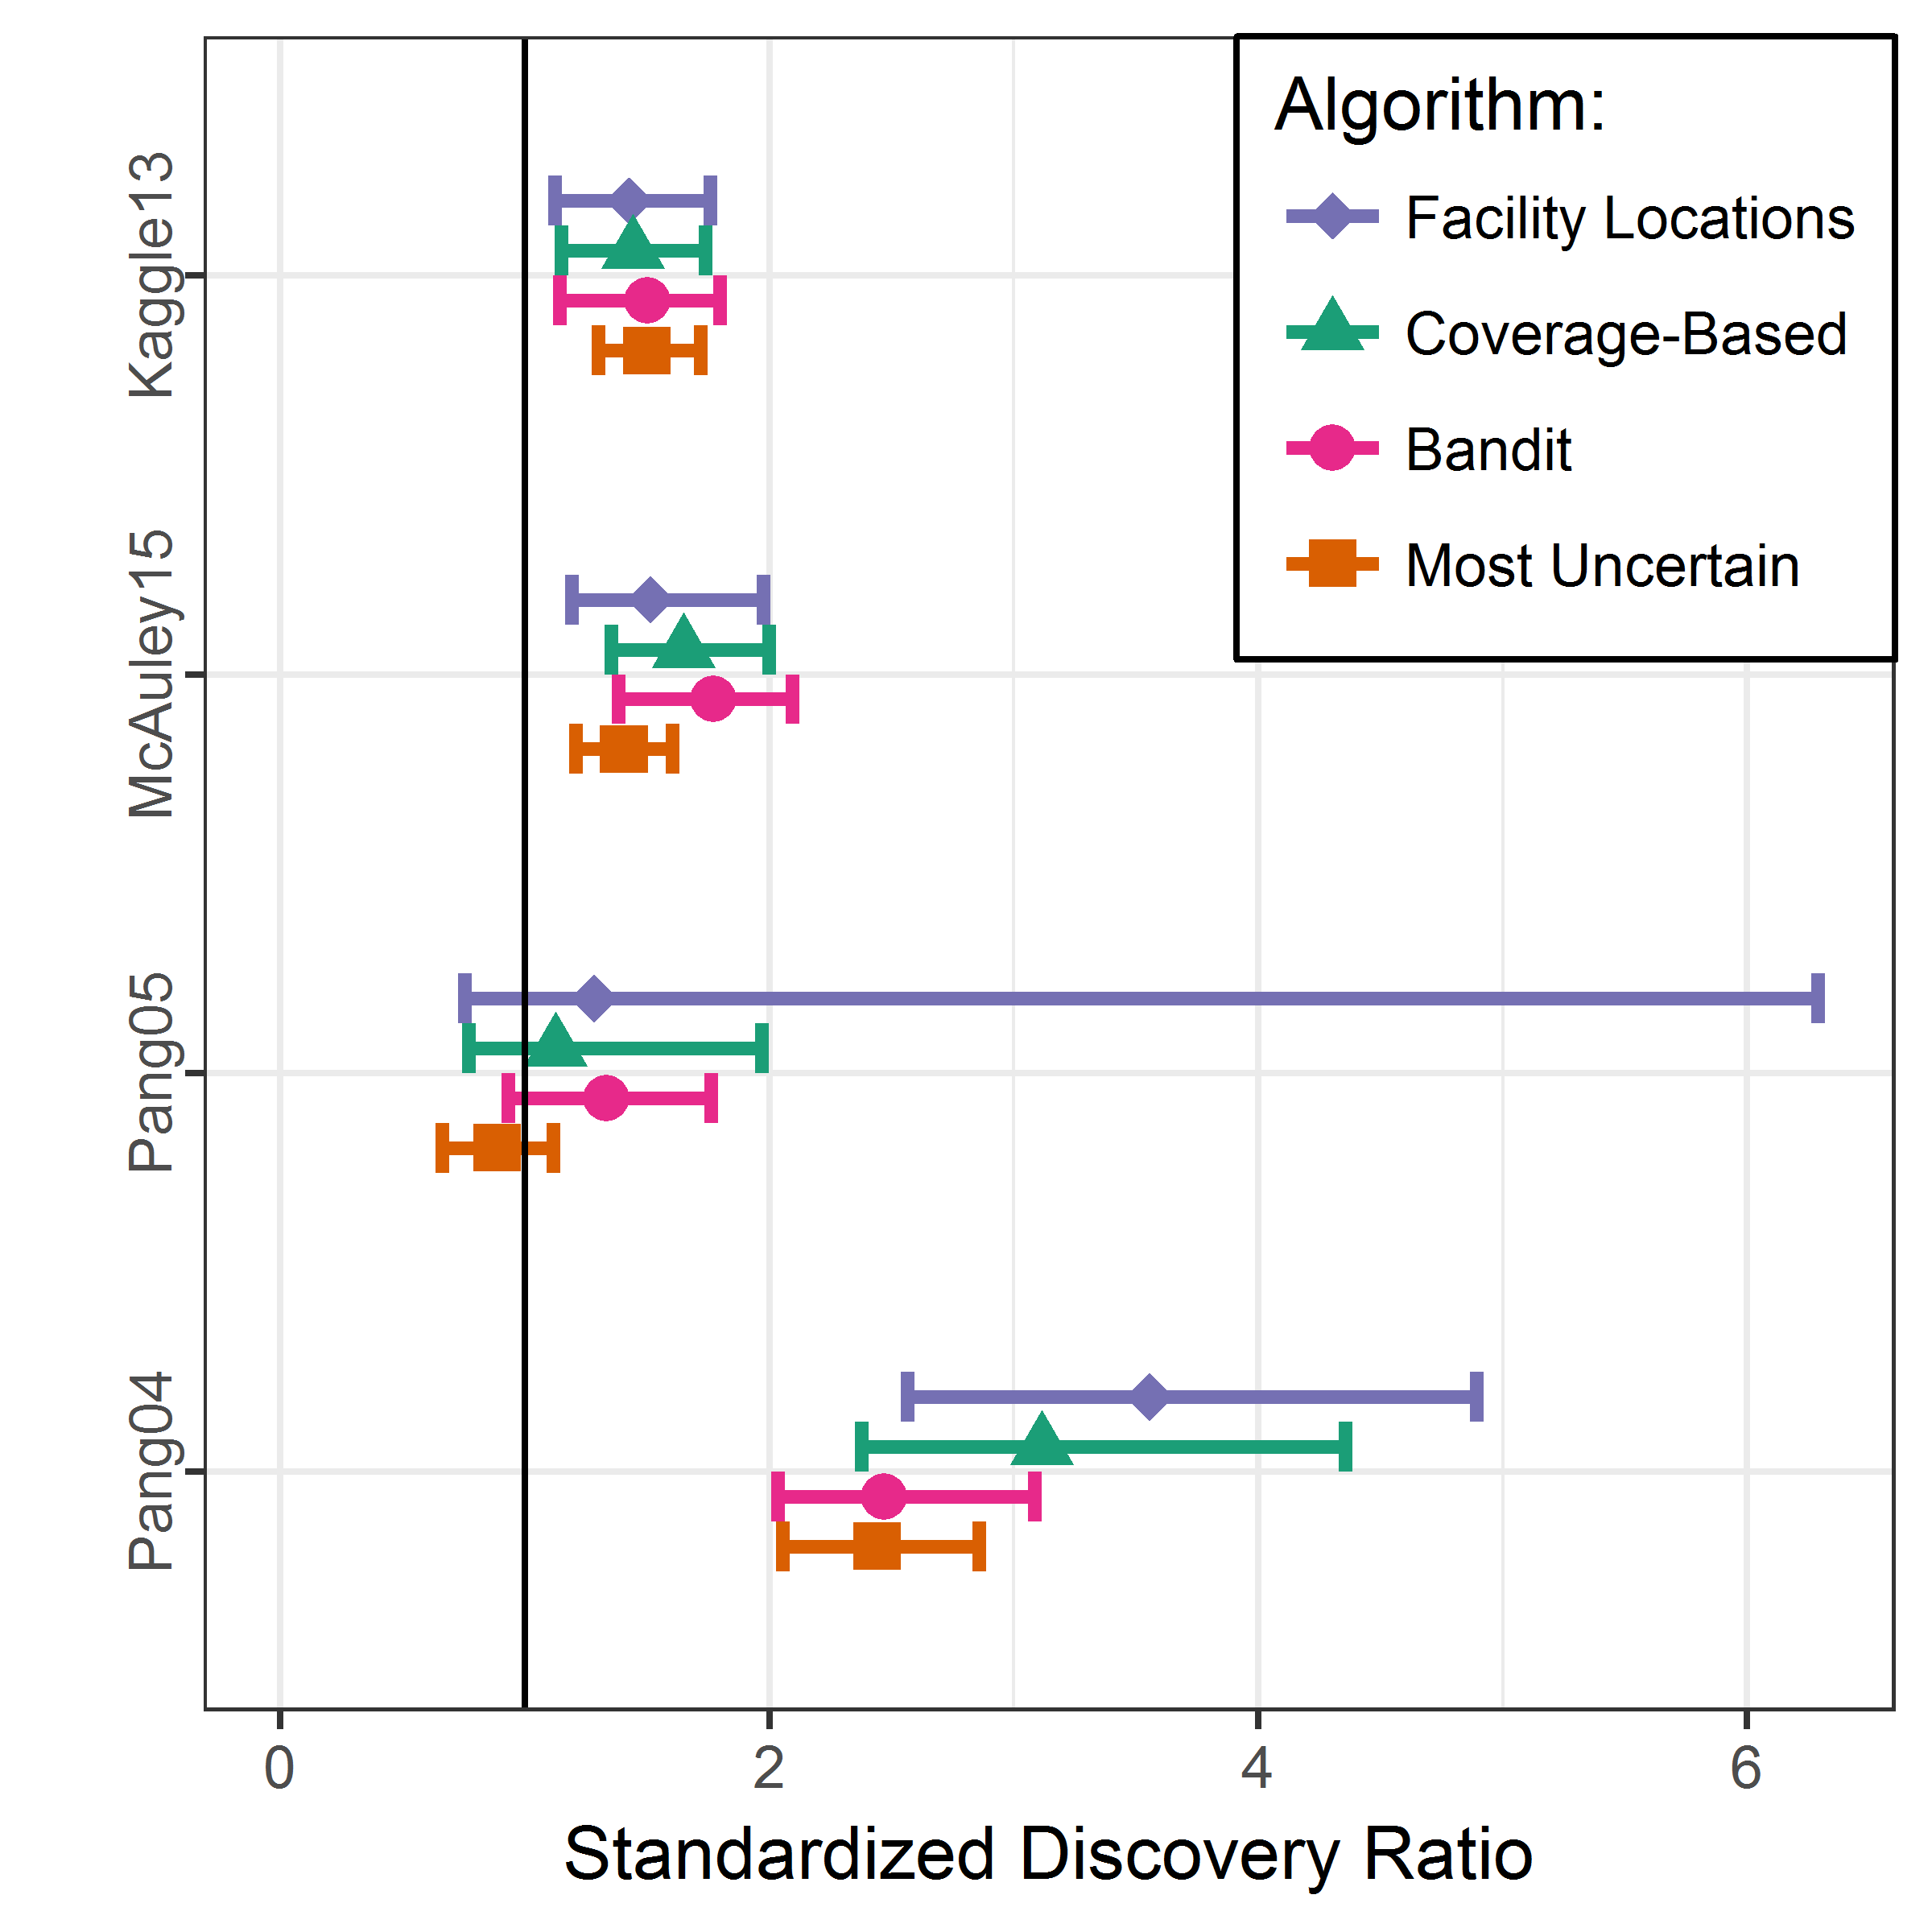
\includegraphics[width=.49\textwidth]{../experimentsAndPlots/discoveryRatioPlaceholder.png}
  \caption{Misclassification Discovery Ratio.}
  \label{fig:discratio}
\end{figure}



\section{Discussion \& Conclusions}

Previous literature has defined unknown unknowns as any highly confident predictions that results in misclassification, but this definition ignores the unavoidable uncertainties of predictive modeling. It should be expected that classifier predictions are imperfect, this is why confidence statements exist! The actions we take as a result of the predictions should take into account the inherent uncertainty. However, in the case where the claimed confidence is overstated, we cannot properly mitigate the risk posed by misclassification. Unlike the previous works that propose utility functions that simply seek to uncover high confidence misclassifications, the facility locations utility that we propose is designed to seek out overconfident misclassifications. We have demonstrated the ability of our greedy algorithm to consistently obtain strong facility locations utility in four data scenarios with disparate overconfidence profiles. 

The use of the logistic regression probability estimates for $\hat{\phi}(x)$ in the optimization step appears to be robust to the underlying structure overconfidence, providing a strong misclassification discovery ratio in the tested cases. This is important because in real-world applications we wouldn’t know the overconfidence behavior a priori to our query search, so we require a versatile estimation method. 

There are many avenues for future work related to the facility locations utility methods that we have presented. First, the facility locations utility model structure separates the discovery reward and coverage proximity components, which could allow separate rescaling to weight each component in line with the priorities of an application. Next, exploratory methods could be developed to evaluate what the query set tells us about the overconfidence of your model, perhaps interpreting the structure of the models used to predict $\hat{\phi}(x)$ to better understand what features are related to overconfidence. Lastly, there may be cases where it is impractical to collect a large enough oracle query set to refit the original classifier, but it may be sufficient to estimate the original classifier’s overconfidence and perform recalibration so that actions taken based on the predictions can include more appropriate risk mitigation. 


\newpage
\bibliographystyle{aaai}

\bibliography{library}


\end{document}
